\documentclass{article}
\usepackage{graphicx} % Required for inserting images
\usepackage{polski}
\usepackage{float}

\title{Rubber Ducky}
\author{Jakub Chuchla, Olaf Sujata, Łukasz Czerwiec, Małgorzata Andrasz}
\date{May 2023}

\begin{document}

\maketitle

\tableofcontents

\section{Słownik}
\begin{itemize}
    \item HID - human input device lub human interface device. Urządzenia służące do wprowadzania danych przez człowieka. Należą do nich między innymi klawiatura, mysz, czy dżojstik.
    \item USB HID - technologia umożliwiająca podłączenie urządzenia do komputera bez konieczności wgrywania sterownika.
    \item HID usage table - tabela definiująca rozłożenie klawiszy klawiatury za pomocą liczb - nie mylić z kodem ASCII.
    \begin{figure}[h]
    \centering
    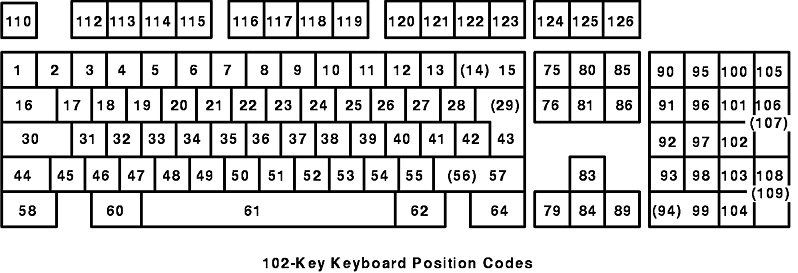
\includegraphics[scale=0.3]{Media/HID.png}
    \caption{Przykładowe rozłożenie klawiszy klawiatury ze zdefiniowanymi wartościami numerycznymi dla każdego z nich}
    \label{fig:enter-label}
    \end{figure}
    
\end{itemize}

\section{Wstęp}

USB Rubber Ducky jest urządzeniem przypominającym pendrive'a, lecz wykrywanym przez komputer, jako urządzenie HID. Należy do kategorii "bad USB", czyli narzędzi, które mają wyrządzić szkodę po podłączeniu do portu USB komputera. Jego twórcą jest Darren Kitchen, który stworzył je, by ukazać słabość modelu zaufania komputera, który po wykryciu USB Rubber Ducky, jako klawiatury, ufa, że to użytkownik komunikuje się z nim poprzez klikanie i pisanie.

Projekt Rubber Ducky ma na celu poznanie sposobu komunikacji z urządzeniami peryferyjnymi. Przygotowaliśmy urządzenie z oprogramowaniem emulującym wciśnięcia klawiszy klawiatury po podłączeniu do komputera przez USB. Zasada działania jest analogiczna do urządzenia Rubber Ducky. 

Rubber to z pozoru przypominające pendrive urządzenie zaliczane jest do kategorii tzw. bad USB, czyli narzędzi, które są nam w stanie wyrządzić jakąś szkodę po podłączeniu do portu USB komputera

\section{Opis działania}

W celu wykorzystania urządzenia USB Rubber Ducky należy je najpierw zaprogramować. Programowanie odbywa się poprzez wgranie napisanego i skompilowanego wcześniej na postać binarną skryptu na umieszczoną w urządzeniu kartę pamięci. Po wgraniu skryptu na USB Rubber Ducky, aby nośnik zadziałał trzeba go podłączyć do portu USB komputera. Po wpięciu do portu USB Rubber Ducky jest wykrywane przez komputer jako klawiatura i zaczyna wysyłać napisane wcześniej ciągi znaków, poleceń i skrótów klawiszowych.

Rubber Ducky, chociaż wygląda jak pamięć flash, w rzeczywistości jest wykrywany przez system operacyjny jako urządzenie HID (Human Interface Device), a konkretnie klawiatura. Po podłączeniu do komputera zaczyna wysyłać zaprogramowane wcześniej ciągi znaków, poleceń i skrótów klawiaturowych. Efekt jest zatem taki, jakby osoba, która podłącza urządzenie do swojego komputera pozwoliła intruzowi skorzystać z własnej klawiatury.

\section{Zagrożenia}

Rubber Ducky niesie ze sobą wiele różnych zagrożeń:
\begin{itemize}
    \item Pozwala stworzyć fałszywe okno logowania do Windowsa wykradając w ten sposób dane logowania lub przesłać wszystkie hasła przeglądarki Chrome na serwer hackera. 
    \item Umożliwiają sprawdzenie do jakiego komputera został podłączony hakerski pendrive - PC czy Mac. Na podstawie otrzymanych informacji, wykonane zostaną polecenia, które będą kompatybilne z danym sprzętem. Ponadto Rubber Ducky może teraz kodować dane w formacie binarnym i przesyłać je wykorzystując sygnały zapalające na klawiaturze lampkę od caps locka.
    \item Kradzież danych logowania - Rubber Ducky może skopiować lub przechwycić wprowadzane dane logowania, takie jak nazwy użytkowników i hasła, które następnie mogą być wykorzystane przez atakującego do uzyskania nieautoryzowanego dostępu do kont i systemów.
    \item Wstrzykiwanie złośliwego kodu - Atakujący może użyć Rubber Ducky do wstrzykiwania złośliwego kodu lub skryptów na zainfekowanym komputerze. Może to prowadzić do instalacji szkodliwego oprogramowania, takiego jak wirusy, trojany czy keylogger'y, które mogą kontrolować system lub kraść dane.
    \item Wykonanie zautomatyzowanych działań - Rubber Ducky może wykorzystać skrypty do wykonywania automatycznych działań, takich jak uruchamianie szkodliwego oprogramowania, przechwytywanie obrazów ekranu, zmiana ustawień systemowych lub przeglądarki, co może prowadzić do utraty prywatności, naruszenia bezpieczeństwa lub poważnych szkód dla użytkownika.
    \item  Przejęcie sesji lub zdalne sterowanie - Atakujący może wykorzystać Rubber Ducky do przejęcia sesji użytkownika lub zdalnego sterowania komputerem, co pozwala im na monitorowanie działań, kradzież danych lub kontrolę nad systemem.
    \item Wprowadzanie zmian w systemie - Rubber Ducky może zmieniać ustawienia systemowe, takie jak firewall, antywirusy czy aktualizacje, aby umożliwić łatwiejsze wdrożenie złośliwego oprogramowania lub uniknąć wykrycia przez zabezpieczenia.
    \item  Atak fizyczny na infrastrukturę - Rubber Ducky może być wykorzystany do przeprowadzenia ataków fizycznych na infrastrukturę, takie jak wstrzykiwanie złośliwego kodu w systemy sterowania przemysłowego, bankomaty lub urządzenia IoT.

    
\end{itemize} 

\section{Działania prewencyjne}

Takie ataki mogą być bardzo groźne dla naszych urządzeń jak i dla nas - ktoś może wykraść dane do logowania, np. do banku.
Oto kilka sposobów, jak możemy bronić nasz komputer przed takimi atakami:
\begin{itemize}
    \item Świadomość i edukacja - dowiedz się więcej o atakach "Rubber Ducky". Wiedza na temat zagrożeń i podstawowych zasad bezpieczeństwa cyfrowego pomoże Ci lepiej rozpoznawać potencjalne zagrożenia i unikać ich.
    \item Uniemożliwienie kontaktu fizycznego z urządzeniem - nie możemy pozwolić na podłączenie pendrive'a nieznanego pochodzenia do naszego komputera. Nie zostawiaj nigdy swojego urządzenia bez opieki w publicznym miejscu.
    \item Zaktualizowane oprogramowanie - Regularnie aktualizuj oprogramowanie na swoim komputerze, w tym system operacyjny, przeglądarkę internetową i inne aplikacje. Aktualizacje często zawierają łatki bezpieczeństwa, które chronią przed znanymi lukami w zabezpieczeniach,
    \item Programy antywirusowe i antymalware - Zainstaluj i regularnie aktualizuj programy antywirusowe i antymalware na swoim komputerze. Skanuj system w poszukiwaniu potencjalnych zagrożeń. Uważaj na ostrzeżenia i blokady, które mogą wskazywać na potencjalne złośliwe oprogramowanie na twoim komputerze.
    \item Firewall - Włącz firewall (zaporę sieciową) na swoim komputerze, aby kontrolować ruch sieciowy i blokować podejrzane połączenia.
    \item Wyłączanie automatycznego uruchamiania - Zablokuj automatyczne uruchamianie skryptów lub programów z urządzeń zewnętrznych, takich jak pendrive'y. Możesz to zrobić, dostosowując ustawienia urządzenia lub oprogramowania do zarządzania urządzeniami pamięci masowej.
    \item Monitorowanie aktywności USB - Jeśli jesteś zaniepokojony możliwością ataku Rubber Ducky, możesz skorzystać z narzędzi monitorujących aktywność na porcie USB, takich jak USBGuard, aby wykryć i zablokować podejrzane działania.
\end{itemize}

Trzeba pamiętać, że żadna metoda nie jest w pełni skuteczna i niezawodna. Dlatego warto stosować kombinację różnych środków ostrożności i zasad bezpieczeństwa cyfrowego, aby jak najlepiej chronić się przed różnymi rodzajami ataków, w tym atakiem Rubber Ducky.

\section{Cel projektu}
Projekt ma na celu poznanie sposobu komunikacji z urządzeniami peryferiów. Stworzyliśmy cztery Rubber Ducky - każde z nich wykonuje inne zadanie, mianowicie:
\begin{itemize}
    \item Pisanie "Hello World" w notatniku w pętli
    \item Stworzenie prostego pliku wsadowego poprzez notatnik, a następnie uruchomienie go
    \item DNS Poisoning poprzez modyfikacje plików systemowych
    \item Wyłączenie rejestrów odpowiedzialnych za porty USB
\end{itemize}
Dokładne opisy napisanych programów można znaleźć w sekcji 8. Napisanie czterech programów o różnych działaniach ma na celu pokazanie w praktyce jak różne zastosowanie może mieć Rubber Ducky.

\section{Sposób implementacji}
\subsection{Geneza wyboru mikrokontrolera}
Wybrany przez nas mikrokontroler to Digispark Attiny 85, pokazany na poniższym zdjęciu obok monety (źródło: https://3d-diy.ru/product/digispark-attiny-85).

\begin{figure}[h]
    \centering
    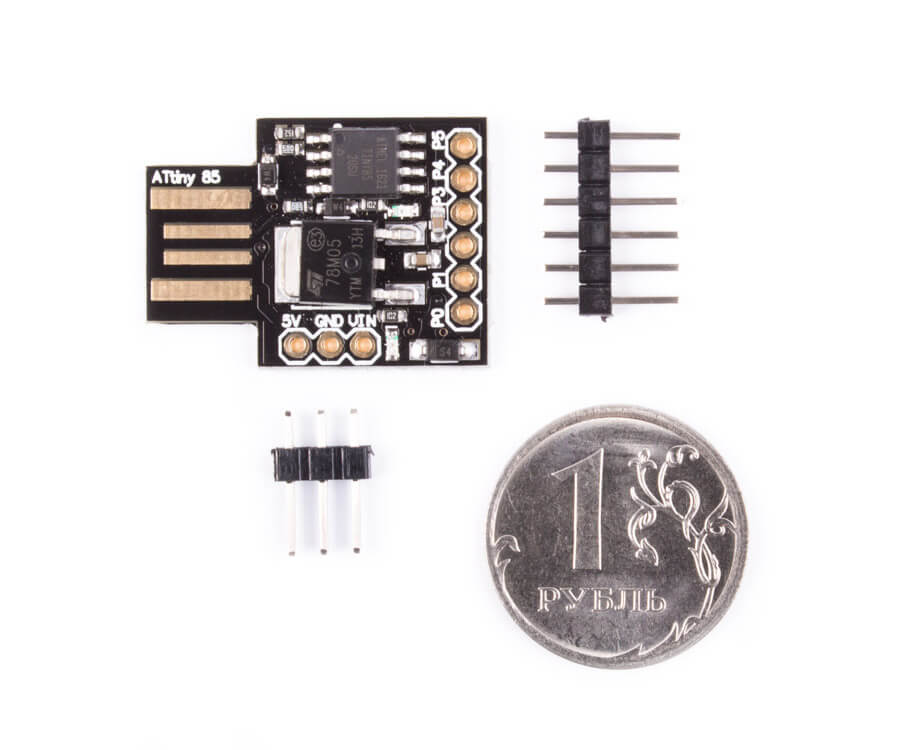
\includegraphics[scale=0.2]{Media/Digispark.jpg}
    \caption{Digispark Attiny 85}
    \label{fig:enter-label}
\end{figure}

Jak widać na powyższym zdjęciu, nasz mikrokontroler jest bardzo mały. Jest to jednym z powodów, przez które został przez nas wybrany. Przez jego wielkość chcieliśmy pokazać, że nawet takie małe urządzenie może być bardzo niebezpieczne. Drobna wielkość wcale nie oznacza, że nasze Rubber Ducky ma mniejsze możliwości - jedynym ograniczeniem była nasza wyobraźnia i wielkość pamięci mikrokontrolera. Kolejnym powodem wyboru tego mikrokontrolera jest fakt, że ma on wbudowane złącze USB, dzięki czemu możemy użyć go jako Rubber Ducky od razu po napisaniu kodu, bez konieczności modyfikowania hardware'u. Wybraliśmy ten mikrokontroler również dlatego, że można o nim łatwo znaleźć dużo informacji oraz jest kompatybilny ze środowiskiem programistycznym Arduino. Na wybór tego mikrokontrolera wpłynęła również jego niska cena.

\subsection{Sposób napisania programów}
W poprzednim podrozdziale wspomnieliśmy, że jednym z powodów wyboru mikrokontrolera była kompatybilność ze środowiskiem programistycznym Arduino. Chcieliśmy napisać nasze programy w tym IDE, ponieważ oprócz tego, że jest popularne, wspierano ono pisanie kodu w języku C++. Wybraliśmy ten język, ponieważ jesteśmy z nim dobrze zaznajomieni i używamy go również na innych kursach znajdujących się w programie naszych studiów.
Kod pisaliśmy używając biblioteki DigiKeyboard.h. Biblioteka ta umożliwiła nam pracę, ponieważ zawarte w niej funkcje pozwalają emulować działanie klawiatury. W bibliotece zdefiniowano wartości znaków odpowiadającym klawiszom klawiatury oraz przyciskom modyfikującym takim jak CTRL, ALT bądź GUI, dzięki czemu nie musieliśmy sami szukać ich w HID usage table. Ważne jest też to, że funkcje w tej bibliotece pozwalają nam na emulowanie kilku klawiszy jednocześnie, ponieważ ze względu na to, że mamy jedynie klawiaturę, musimy używać skrótów klawiszowych systemu Windows, żeby móc zapisać i włączyć napisany przez nas skrypt na komputerze do którego podłączymy nasze Rubber Ducky.
W napisanych przez nas programach używamy funkcji delay, która każe skryptowi zaczekać przed wykonaniem dalszych instrukcji. Jest to ważne, by Rubber Ducky działało niezawodnie. Niektóre komputery mogą potrzebować trochę więcej czasu na przetworzenie danych wysyłanych przez klawiaturę. Dzięki zaczekaniu chwili przed "wciśnięciem" kolejnych klawiszy mamy pewność, że poprzednia akcja zostanie obsłużona przed próbą wykonania kolejnej - daje nam to pewność poprawnego wykonania się wszystkich instrukcji. System może mieć również problem z przepustowością przetwarzania danych z klawiatury, przez co przy zbyt szybkim wysłaniu zbyt wielu poleceń, któreś może się nie wykonać. 

\subsection{Napotkane problemy}
\begin{itemize}
    \item Pierwszym problemem jaki napotkaliśmy była instalacja sterowników do naszego mikrokontrolera, ale po krótkiej "zabawie" z nimi, mogliśmy zacząć pisać kod. 
    \item Kolejny problem pojawił się przy próbie wypisania podanego tekstu na ekran przy użyciu funkcji println. Po przeanalizowaniu napisanego kodu oraz tabeli ASCII okazało się, że mikrokontroler wyświetla znaki cofnięte o wartość 8 w kodzie ASCII, więc przy wyświetlaniu tekstów musimy dodać tę wartość do każdego ze znaków. Błąd naprawiliśmy używając pętli for. Mylne działanie instrukcji wynika prawdopodobnie z tego, że instrukcja println nie jest zdefiniowana w bibliotece DigiKeyboard.h, lecz w bibliotece Print, która jest dziedziczona przez DigiKeyboard.h. Pomimo jej mylnego działania umożliwia nam ona przesyłanie długich ciągów znaków (string) co bardzo ułatwia pisanie kodu.
    %Chuchla
    \item Nie wszystkie przyciski były zdefiniowane w bibliotece DigiKeyboard.h, a ich użycie było niezbędne do poprawnego działania skryptu. By poradzić sobie z problemem znaleźliśmy odpowiadające wartości takowych przycisków w HID Usage Table. Przykładowo "strzałce w dół" odpowiadają wartości 81/0x51. Przez wysłanie "stroke'a" takiej wartości (dziesiętnej/szesnastkowej) otrzymywaliśmy zamierzony efekt.
    \item Brak wystarczającej ilości pamięci w mikrokontrolerze. Wybraliśmy to urządzenie ze względów opisanych wcześniej (Rozdział 7.1) - problem wynikł podczas tworzenia oprogramowania nr 2, gdzie poprzednim celem było "narysowanie" czegoś w notatniku używając technik textArt. Niestety wielkość całego programu "przerosła" nasz malutki mikrokontroler, skutkiem czego było porzucenie tego pomysłu oraz konieczność nauczenia się pisania programów bardziej "pamięcioszędnych".
\end{itemize}




\section{Opis działania programów}
\subsection{Program 1 - Hello World}
    \begin{itemize}
        \item Działanie - Program uruchamia notatnik, następnie w pętli wypisuje "Hello World".
        \item Cel - Zapoznanie Nas z najbardziej podstawową rzeczą jaką jest w stanie zrobić Rubber Ducky czyli wypisanie "czegoś" na ekranie.
        \item Wnioski - Program w początkowych fazach rozwoju projektu, służył głównie do rozpoznania czy nasz "pendrive" po podpięciu go do portu USB wykrywany jest poprawnie oraz czy działa według naszych założeń. Na większość napotkanych problemów (Rozdział 7.3), z którymi zderzyliśmy się podczas tworzenia projektu natrafiliśmy podczas testów na tym programie. Pozwolił nam on na dopracowanie działania naszego urządzenia oraz rozwiązaniu błędów związanych z jego działaniem.    
    \end{itemize}
\subsection{Program 2 - \%random\%.bat}
    \begin{itemize}
        \item Działanie - Program uruchamia notatnik, następnie tworzy prosty plik Batch, który ma za zadanie wyświetlać w nieskończoność losowe liczby na ekranie.
        \item Cel - Poznanie prostej składni plików wsadowych, stworzenie prostego skryptu oraz odpalenie go z poziomu pulpitu.
        \item Wnioski - Po stworzeniu programu potrafiliśmy już zapisywać i odpalać  programy z poziomu pulpitu użytkownika komputera. Zyskaliśmy informacje na temat plików typu Batch oraz kilku skrótów klawiszowych potrzebnych do zakładanego działania naszego Rubber Ducky. Wiedza zdobyta podczas wytwarzania danego oprogramowania poszerzyła nasze horyzonty związane z potencjałem jaki drzemie w naszym Rubber Ducky oraz samej klawiaturze. Dowiedzieliśmy się, że bardzo prosty skrypt Batch byłby w stanie doprowadzić komputer do stanu nieużywalności.
    
    \end{itemize}
\subsection{Program 3 - DNS Poisoning}
    \begin{itemize}
        \item Działanie - Program uruchamia notatnik w trybie administratora, następie otwiera plik hosts, w którym podaje ip, na które ma zostać przekierowany użytkownik po wpisaniu adresu facebook.com w przeglądarce - w tym przypadku jest to ip strony Microsoft. Następnie zapisuje wszystkie zmiany oraz wyłącza notatnik.
        \begin{figure}[h]
    \centering
    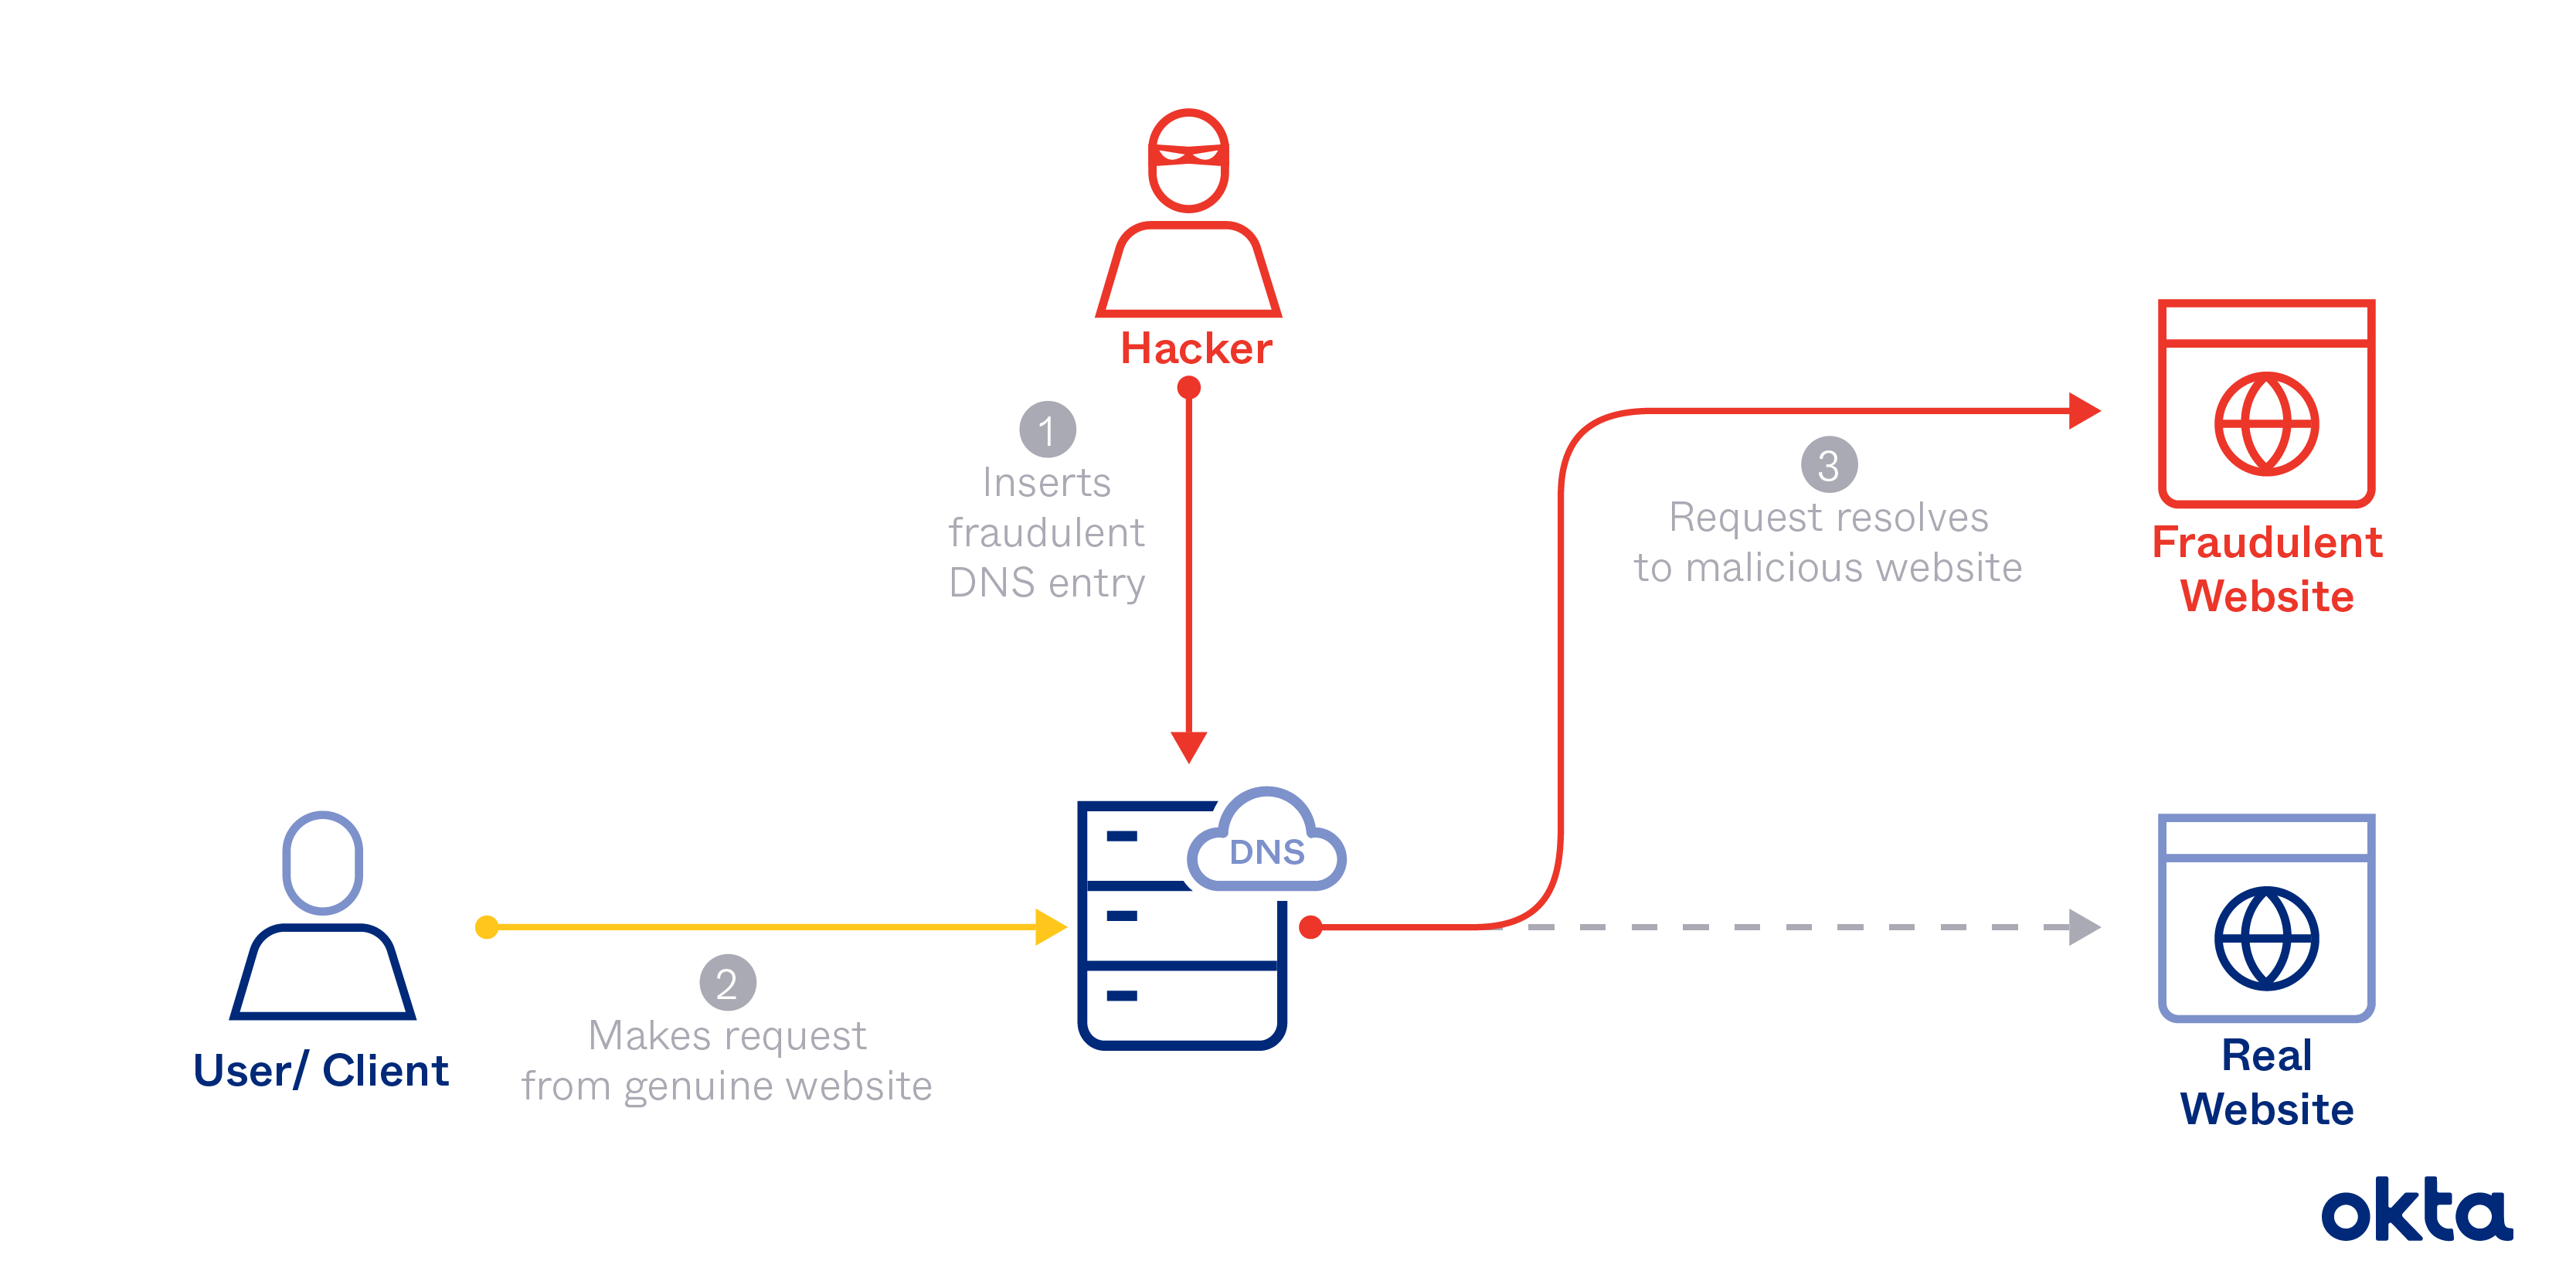
\includegraphics[scale=0.1]{Media/DNS1.png}
    \caption{Grafika przedstawiająca działanie ataku DNS Poisoning}
    \label{fig:enter-label}
    \end{figure}
        \item Cel - Stworzenie programu, który przybliży nasze urządzenie do miana "Rubber Ducky". Oprogramowanie w widoczny sposób wpłynie na zachowanie komputera oraz utrudni korzystanie z niego użytkownikowi.
        \item Wnioski - Nauczyliśmy się następnych skrótów klawiszowych potrzebnych do założonego działania naszego urządzenia. Mimo, że program działa bez zarzutów to dzisiejsze zabezpieczenia wbudowane w przeglądarkę uniemożliwiają nam uzyskanie efektów, które 7/8 lat temu byłby możliwe do osiągnięcia przez niższe standardy bezpieczeństwa. Przeglądarki wykrywają naszą próbę przekierowania użytkownika na "zły" adres ip i blokują połączenie ze stroną mimo, że jest ona bezpieczna (microsoft.com). Niemniej jednak osoba bez wiedzy związanej z takimi atakami mogłaby nie doszukać się źródła problemu jakim jest modyfikacja jego plików Windows. Strona microsoft.com nie wyświetli się lecz witryna, na którą użytkownik chciał się początkowo dostać również będzie dla niego niedostępna. Załączone zdjęcie (Rysunek 4) będzie jednak dowodem, że nasz program działa - po próbie wejścia na witrynę facebook.com wyświetlany jest certyfikat strony microsoft.com.
        \begin{figure}[h]
    \centering
    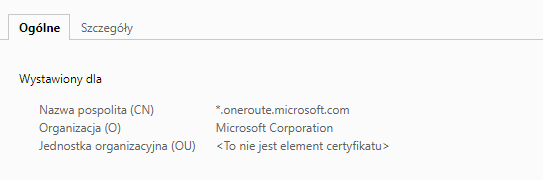
\includegraphics[scale=0.5]{Media/DNS.png}
    \caption{Grafika przedstawiająca działanie ataku DNS Poisoning}
    \label{fig:enter-label}
    \end{figure}
    \end{itemize}    
\subsection{Program 4 - USB Disabler}
    \begin{itemize}
        \item Działanie - Program uruchamia notatnik w trybie administratora, następnie tworzy plik Batch, którego zadaniem jest modyfikacja działania rejestru USBHUB3 - ustawia wartość klucza start na 4 co powoduje nie włączenie się rejestru po ponownym uruchomieniu komputera co skrypt również robi. Po stworzeniu pliku jest on uruchamiany z poziomu pulpitu w trybie administratora.
        \item Cel - Stworzenie programu, który zmieni działanie komputera w taki sposób, że użytkownik straci nad nim kontrole w całkowitym bądź częściowym stopniu.
        \item Wnioski - Tworząc ten program musieliśmy poszerzyć naszą ogólną wiedze związaną z tematem rejestrów w Systemie Windows. Przeprowadziliśmy testy, które polegały głównie na metodzie prób i błędów - "wyłączaliśmy" różne rejestry tak by osiągnąć zamierzony efekt czyli pozbyć się sygnału w portach USB (Rysunek 5). Uznaliśmy, że dobrym pomysłem byłoby po prostu wyłączenie wszystkich rejestrów odpowiedzialnych za porty USB tj. USBHUB, USBHUB3, USBEHCI, USBSTOR itd., lecz znów natknęliśmy na problem z niewystarczającą ilością pamięci w mikrokontrolerze. Niestety skrypt był za długi i urządzenie by go nie "udźwignęło". Nie chcieliśmy zaniechać tego pomysłu, więc "wstrzeliliśmy się" w odpowiedni rejestr i uzyskaliśmy zamierzony efekt - przynajmniej dla portów USB3.
        \begin{figure}[h]
    \centering
    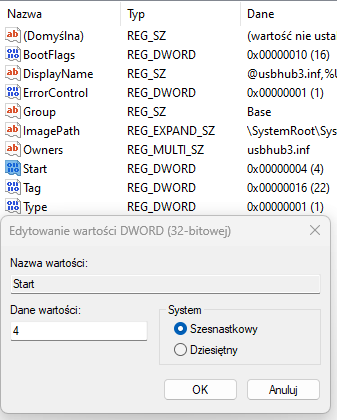
\includegraphics[scale=0.4]{Media/Rejestr.png}
    \caption{Rejestr USBHUB3 - ustawienie wartości start na 4 czyli tryb "disable"}
    \label{fig:enter-label}
    \end{figure}
    \begin{figure}[h]
    \centering
    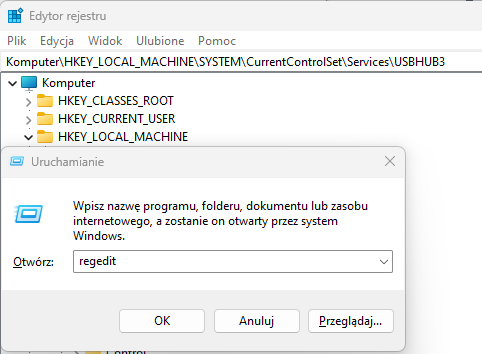
\includegraphics[scale=0.5]{Media/Rejestr1.png}
    \caption{Sposób dostania się do edytora rejestrów oraz ścieżka prowadząca do rejestru USBHUB3}
    \label{fig:enter-label}
    \end{figure}
    \end{itemize} 
    
        

\section{Wnioski}


\section{Podsumowanie}


\begin{thebibliography}{9}

\bibitem{}
  https://opensecurity.pl/arsenal-ethical-hackera-rubber-ducky/
 \bibitem{} https://www.komputerswiat.pl/aktualnosci/bezpieczenstwo/falszywy-hakerski-pendrive-stal-sie-jeszcze-grozniejszy-jest-jeden-sposob-zeby-sie/7l4v3re
 \bibitem{} https://chat.openai.com/
 \bibitem{} https://github.com/digistump/DigisparkArduinoIntegration/blob/master/libraries/DigisparkKeyboard/DigiKeyboard.h
 \bibitem{} https://securitydiaries.com/11-insane-things-can-batch-programming/
 \bibitem{} https://www.okta.com/identity-101/dns-poisoning/
 \bibitem{} https://support.microsoft.com/en-us/topic/how-can-i-prevent-users-from-connecting-to-a-usb-storage-device-460ef516-8ac8-07af-e90b-0d9ac55bcd4d
\end{thebibliography}

\end{document}

